\documentclass[a4paper, 11pt,oneside]{article}
\usepackage[
  top=1.5cm,
  bottom=1cm,
  left=2cm,
  right=1.5cm,
  headheight=25.22153pt, % as per the warning by fancyhdr
  includehead,includefoot,
  heightrounded, % to avoid spurious underfull messages
]{geometry} 

\usepackage[T1]{fontenc}
\usepackage{microtype}
\usepackage{fancyhdr}
\usepackage{fancyvrb}
\usepackage{lipsum}
\usepackage{url}
\usepackage{listings}
\usepackage{lastpage}
\usepackage{enumitem}
\usepackage{datetime}
\usepackage{amsthm}
\usepackage{graphicx}
\usepackage{hyperref}
\usepackage{minted}
\usepackage{float}

\settimeformat{hhmmsstime}
\yyyymmdddate

\pagestyle{fancy}
\fancyhf{} % clear all fields

\pagestyle{fancy}
\lhead{CMSC 132: Computer Architecture \\ First Semester 2020-2021}
\rhead{$\copyright$Institute of Computer Science \\ University of the 
Philippines Los Banos}
\rfoot{JACHermocilla (CC NC-BY-SA 4.0)}
%\cfoot{Enjoy!:)}
\cfoot{\thepage\ of \pageref{LastPage}}
\lfoot{Revision: \today\ \currenttime}
%\rfoot{https://jachermocilla.org/teaching/125}
\renewcommand{\headrulewidth}{0.4pt}
\renewcommand{\footrulewidth}{0.4pt}

\begin{document}

\begin{center}
	{\LARGE \textbf{Sequential Logic Circuits}}
\end{center}

\section*{Learning Outcomes}
   At the end of this lab, you should be able to:
   \begin{enumerate}[itemsep=0pt,parsep=0pt]
   	   \item differentiate combinational and sequential elements in a processor;
       \item implement sequential logic circuit elements in VHDL;
   \end{enumerate}   
\tableofcontents

\section{Resources}
\begin{itemize}
	\item Video: \href{https://youtu.be/CzyXb_T-xgU}{https://youtu.be/CzyXb\_T-xgU}.
	\item Source Codes: \href{https://git.io/JU3al}{https://git.io/JU3al}
	\item Online VHDL Tool: \href{https://www.edaplayground.com/home}
	{https://www.edaplayground.com/home}
\end{itemize}	

\section{Discussion}
The discussion in this handout aims only to provide an outline of what is in 
the video lecture. It is recommended that you watch the video in its entirety.

Sequential elements are sometimes called memory elements because they store 
state information. The\textit{ output} of any memory element dependes on both 
the \textit{input} and the \textit{value stored} in it. An understanding of 
clocks is important in the study of sequential elements. 

\subsection{Clocks}
Clocks determine when the current state of a sequential elements needs to be
updated. It is a \textit{signal} that transitions from low to high and high to
low in a fixed cycle time or clock period. Figure \ref{fig:clock0} shows an
example clock signal. It is a digital signal so it is represented by a square 
wave and the transition from low to high or high to low is abrupt unlike in 
analog signals. These abrupt transitions are called \textit{clock edges} which 
may be a \textit{rising edge} (low to high) or \textit{falling edge} (high to
low). The \textit{clock period} is the time to complete a cycle and the number 
of cycles per second is called the \textit{frequency} in \textit{hertz}. The 
higher the frequency the higher the number of cycles per second. We will use 
these parameters later when we go to the performance evaluation lab. 

\begin{figure}[H]
	\begin{center}
	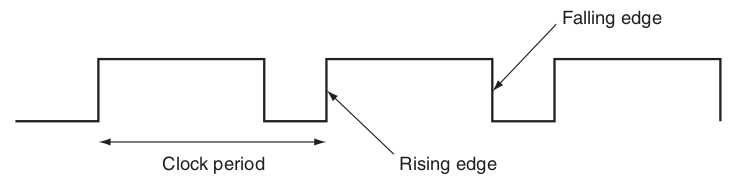
\includegraphics[width=4in]{clock0.png}
	\caption{A clock signal showin the clock period, falling edge, and rising edge.}
	\label{fig:clock0} 
	\end{center}
\end{figure}

The updating of state elements is usually done at clock edge to ensure that the 
signals will be valid. Figure \ref{fig:clock1} shows a combinational element 
sandwiched between two state elements. Observe that the updating of the state 
elements is done at the rising edge. Using the clock edge as marker allows the 
same state element to be the input and output of the combinational element, 
without invalidating the signal. 

\begin{figure}[H]
	\begin{center}
	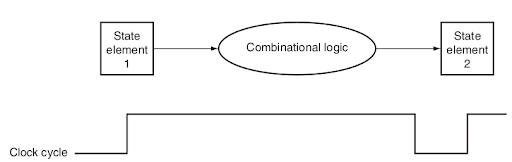
\includegraphics[width=4in]{clock1.png}
	\caption{A combinational element is sandwiched between two state elements. 
	The state elements are updated at the rising clock edge.}
	\label{fig:clock1} 
	\end{center}
\end{figure}

The VHDL code below shows how to generate a clock signal \textit{clk} that can 
be used in a testbench as input to sequential elements being tested. 

\begin{minted}[frame=single,framesep=10pt]{vhdl}
LIBRARY ieee;
USE ieee.std_logic_1164.all;
ENTITY clocker_tb IS
END clocker_tb;
ARCHITECTURE behavior OF clocker_tb IS
   --100Mhz
   CONSTANT frequency: integer := 100e6; 
   CONSTANT period : time := 1000 ms / frequency;
   SIGNAL clk : std_logic := '0';
BEGIN 
   clk <= not clk after period / 2;
   -- do some stuff here using clk as input
END ARCHITECTURE;
\end{minted}

\subsection{Latches}
Latches are unclocked memory elements. Figure \ref{fig:latch0} shows a
Set-Reset(SR) latch using two NOR gates. Q is the main output and Q bar is the 
complement of Q. When Q is true, if S is asserted then Q will be asserted. 
When R is asserted, then Q bar will be asserted. 

\begin{figure}[H]
	\begin{center}
	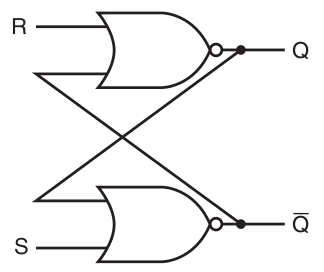
\includegraphics[width=2in]{latch0.png}
	\caption{A Set-Reset latch.}
	\label{fig:latch0} 
	\end{center}
\end{figure}

The code VHDL code for the S-R latch is shown below.

\begin{minted}[frame=single,framesep=10pt]{vhdl}
LIBRARY ieee;
USE ieee.std_logic_1164.all;
---------------------------------
ENTITY sr_latch IS
   PORT (R, S: IN STD_LOGIC;
   Q, Q_BAR: INOUT STD_LOGIC);
END sr_latch;
--------------------------------
ARCHITECTURE pure_logic OF sr_latch IS
BEGIN
   Q <= R NOR Q_BAR;
   Q_BAR <= S NOR Q;
END pure_logic;
\end{minted}

When a clock is added to a latch, it is called a clocked latch. Figure 
\ref{fig:latch1} shows a D latch. The clock input is C and the data input is D. 
Q is the internal state. It is basically an extension of the S-R latch. An
important thing to remember is that in clocked latches, \textit{the state 
changes whenever the input change and the clock is asserted}.

\begin{figure}[H]
	\begin{center}
	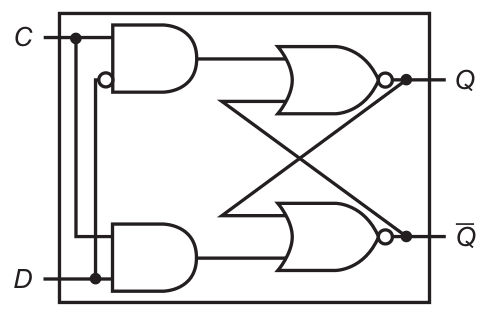
\includegraphics[width=2.5in]{latch1.png}
	\caption{A D latch. }
	\label{fig:latch1} 
	\end{center}
\end{figure}

The VHDL code for the D latch is shown below. 

\begin{minted}[frame=single,framesep=10pt]{vhdl}
LIBRARY ieee;
USE ieee.std_logic_1164.all;
---------------------------------
ENTITY d_latch IS
   PORT (C, D: IN STD_LOGIC;
   Q, Q_BAR: INOUT STD_LOGIC);
END d_latch;
--------------------------------
ARCHITECTURE pure_logic OF d_latch IS
BEGIN
   Q <= (C AND NOT D) NOR Q_BAR;
   Q_BAR <= (D AND C) NOR Q;
END pure_logic;
\end{minted}

\subsection{Flip-Flops}
Flip-flops are similar to clocked-latches. The main difference is the 
update of the state happens at the edge of the clock signal. Recall the
advantage of edge-triggered clocking methodology above. Figure \ref{fig:dff0} 
shows a D flip-flop using D latches.

\begin{figure}[H]
	\begin{center}
	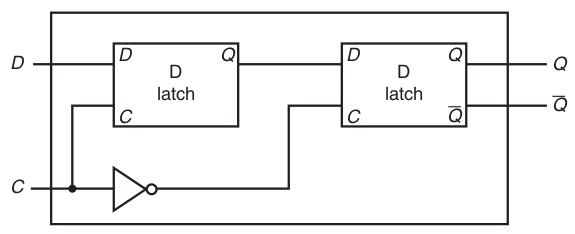
\includegraphics[width=4in]{dff0.png}
	\caption{A D flip-flop created using two D latches in a master-slave 
	configuration.}
	\label{fig:dff0} 
	\end{center}
\end{figure}

The VHDL code for this D flip-flop is shown below. There is a simpler code for
this described in the video.

\begin{minted}[frame=single,framesep=10pt]{vhdl}
LIBRARY ieee;
USE ieee.std_logic_1164.ALL;
ENTITY dff is
   PORT( D: IN STD_LOGIC;
      C: IN STD_LOGIC;
      Q: INOUT STD_LOGIC;
      Q_BAR: INOUT STD_LOGIC);
END dff;
ARCHITECTURE behavioral OF dff IS
   COMPONENT d_latch IS
      PORT (C, D: IN STD_LOGIC;
      Q, Q_BAR: INOUT STD_LOGIC);
   END COMPONENT;
   SIGNAL u,v: STD_LOGIC;
   SIGNAL NOTC: STD_LOGIC := NOT C;
BEGIN
   master: d_latch port map (C, D, u, v);
   slave: d_latch port map (NOTC, u, Q, Q_BAR);
END behavioral;
\end{minted}

\subsection{Register Files}
A register file consists of a set of registers that can be read and written by
supplying a register number to be accessed. Figure \ref{fig:rf0} shows an 
example register file where two registers can be read and one register can be 
written into. In order to write to a register, the \textit{Write} enable
control signal should be asserted.

\begin{figure}[H]
	\begin{center}
	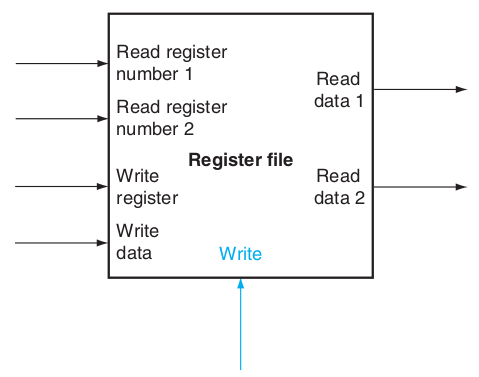
\includegraphics[width=3in]{rf0.png}
	\caption{2-to-1 Multiplexer.}
	\label{fig:rf0} 
	\end{center}
\end{figure}

Registers are implemented as flip-flops. A multiplexer is used to select which
register output will be allowed to pass through during read. Figure 
\ref{fig:rf1} shows two multiplexers connected to the array of registers because
the register file allows two registers to be read.

\begin{figure}[H]
	\begin{center}
	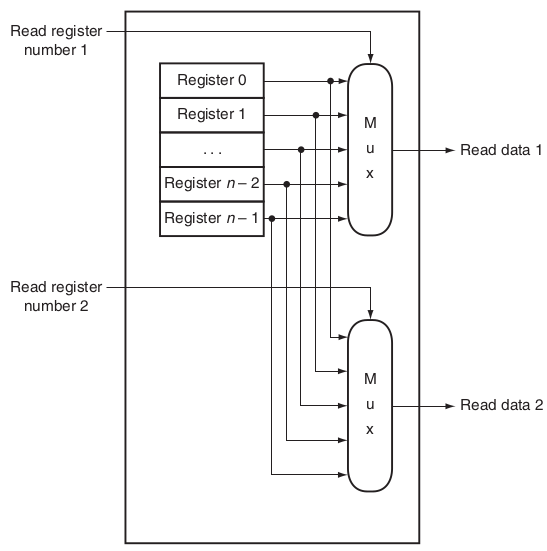
\includegraphics[width=4in]{rf1.png}
	\caption{Reading in a register file.}
	\label{fig:rf1} 
	\end{center}
\end{figure}

Writing to a register file will require a decoder to select the register to 
write to. The output of the decoder is and-ed to the\textit{Write} control 
signal. The result is used as the clock input to the register(flip-flop) as 
shown in Figure \ref{fig:rf2}. 

\begin{figure}[H]
	\begin{center}
	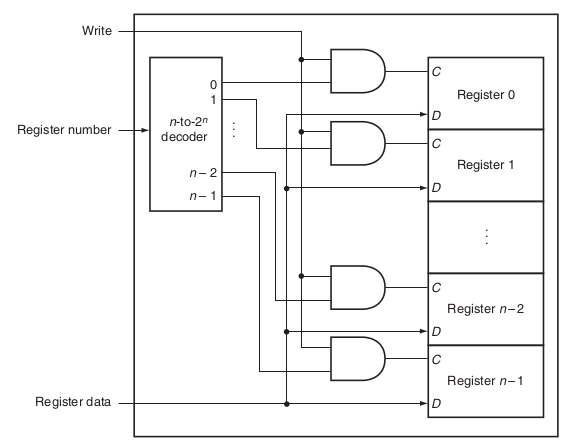
\includegraphics[width=4in]{rf2.png}
	\caption{Writing to a register file.}
	\label{fig:rf2} 
	\end{center}
\end{figure}

The VHDL source code for a register file with 2 1-bit registers is shown below. 
The \textit{registers} signal is defined as an array type. The register numbers
are used as index into this array.  
\begin{minted}[frame=single,framesep=10pt]{vhdl}
LIBRARY ieee;
USE ieee.std_logic_1164.ALL;
USE IEEE.NUMERIC_STD.ALL;

ENTITY reg_file2 is
   PORT( 
      read_n1: IN STD_LOGIC;
      read_n2: IN STD_LOGIC;
      write_n: IN STD_LOGIC;
      write_data: IN STD_LOGIC;
      write: IN STD_LOGIC;
      clk: IN STD_LOGIC;
      read_data1: OUT STD_LOGIC;
      read_data2: OUT STD_LOGIC);
END reg_file2;
ARCHITECTURE behavioral OF reg_file2 IS
TYPE rf_type IS ARRAY(0 to 1) of STD_LOGIC;
SIGNAL registers : rf_type;
BEGIN
   rf: PROCESS(clk)
   BEGIN
      IF RISING_EDGE(clk) THEN
         IF (write ='1') THEN
            registers(TO_INTEGER(UNSIGNED'('0' & write_n))) <= write_data;
         END IF;
      END IF;
      read_data1 <= registers(TO_INTEGER(UNSIGNED'( '0' & read_n1)));
      read_data2 <= registers(TO_INTEGER(UNSIGNED'( '0' & read_n2)));
   END PROCESS;
END behavioral;
\end{minted}

Registers are fast memory elements but has limited storage. For example, in the 
Intel x86\_64 processor, the size of the the registers is 64-bits. For larger 
storage, Random Access Memory (RAMs) is used. 


\subsection{Static RAM}
Static RAM (SRAM) has a specific configuration in terms of the \textit{number 
of 
addressable locations} and \textit{width of each addressable location}. Figure 
\ref{fig:sram0} shows an SRAM with 2M addressable locations and each
location is 16 bits. The address line is 21 bits and the data input and output 
is 16 bits.

\begin{figure}[H]
	\begin{center}
	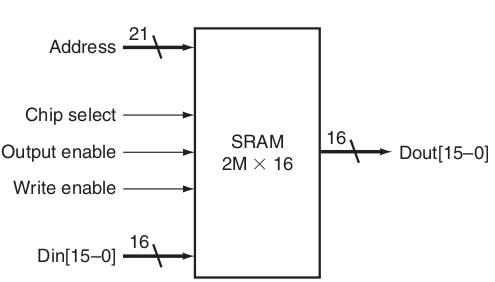
\includegraphics[width=3in]{sram0.png}
	\caption{A 2Mx16 SRAM.}
	\label{fig:sram0} 
	\end{center}
\end{figure}

Since SRAMs can store large amount of information, using a multiplexer to 
select the location is not cost-effective. Instead, a shared output line, called
a \textit{bit line}, allows multiple memory cells in the memory array to
assert. The circuitry to allow enable this is called the 
\textit{three-state buffer} or \textit{tristate buffer} 
(Figure \ref{fig:sram1}).

\begin{figure}[H]
	\begin{center}
	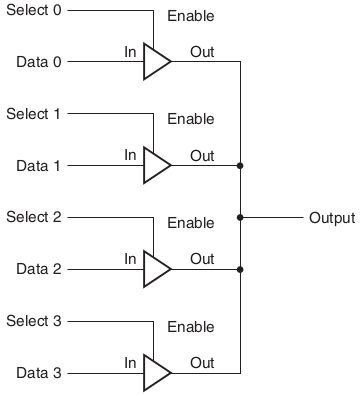
\includegraphics[width=3in]{sram1.png}
	\caption{Tristate buffer allows multiple memory cells to share a bit line 
	making it more cost-effective than using a multiplexer.}
	\label{fig:sram1} 
	\end{center}
\end{figure}

The VHDL code for the D flip-flop with the \textit{Enable} line and 
\textit{Reset} line is shown below. 

\begin{minted}[frame=single,framesep=10pt]{vhdl}
LIBRARY ieee;
USE ieee.std_logic_1164.all;

ENTITY DFF is
PORT( din: IN STD_LOGIC;
      clk: IN STD_LOGIC;
      rst: IN STD_LOGIC;
      en: IN STD_LOGIC;
      dout: OUT STD_LOGIC);
END DFF;

ARCHITECTURE behavioral of DFF is
BEGIN
   PROCESS(rst,clk,din)
      BEGIN
         IF (rst='1') THEN
            dout<='0';
         ELSIF(RISING_EDGE(clk)) THEN
            IF (en='1') THEN
               dout<= din;
            ELSE
               dout<='Z';
            END IF;
      END IF;
   END PROCESS;
END behavioral;
\end{minted}


A small 4x2 SRAM might be built using D latches with an \textit{Enable} line as 
shown in Figure \ref{fig:sram3}. 

\begin{figure}[H]
	\begin{center}
	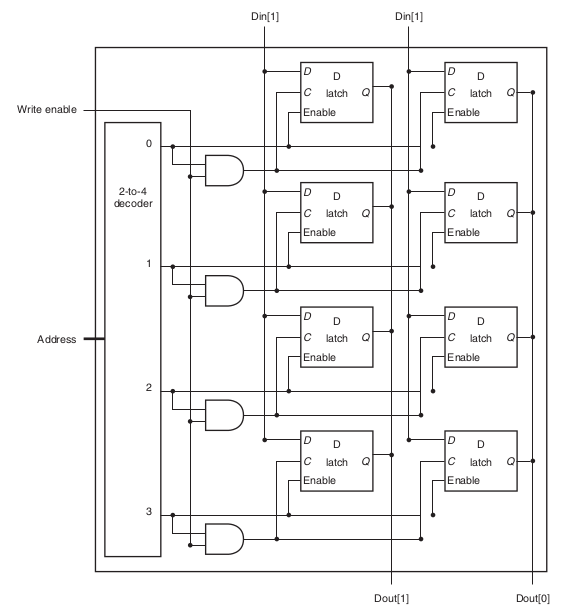
\includegraphics[width=3.5in]{sram3.png}
	\caption{A 4x2 SRAM.}
	\label{fig:sram3} 
	\end{center}
\end{figure}

To reduce the size of the decoder, SRAMs use a two-step decoding method. In 
Figure \ref{fig:sram2}, the first decoder generates the addresses for an eight 
4K x 1024 arrays then a set of multiplexers is used to select 1 bit from each 
1024-bit-wide array. The address lines are split into two groups.

\begin{figure}[H]
	\begin{center}
	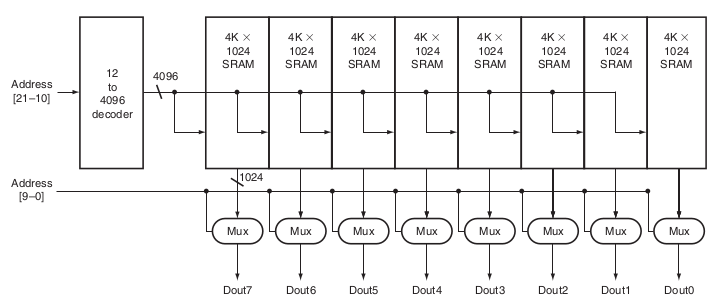
\includegraphics[width=5in]{sram2.png}
	\caption{Two-step decoding to reduce the size of the decoder in SRAM.}
	\label{fig:sram2} 
	\end{center}
\end{figure}

\subsection{Dynamic RAM}
The values in SRAM are stored in the flip-flops. As long as there is power, the
values stored can be kept indefinitely. In Dynamic RAM (DRAM), the values are 
stored as charge in a capacitor. It uses a single transistor to access the
the values. SRAMs require four to six transistors per bit, thus DRAMs are much 
cheaper for use in main memory. SRAMs are usually used for caches. The main 
drawback for DRAMs is that it must periodically be refreshed (read the 
values then write again), thus the word \textit{dynamic}. DRAMs use two-level 
decoding consisting of a row access followed by a column access.  
Figure \ref{fig:dram0} shows a 4Mx1 DRAM. Notice that a single  address line is
used to for both the row and column access. A pair of signals are used to tell 
whether the value in the address line is for row or column. See Further Reading
section on a simple implementation of RAM in VHDL.  

\begin{figure}[H]
	\begin{center}
	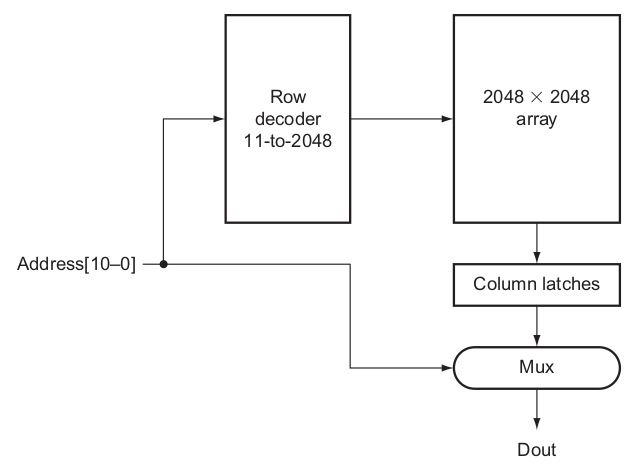
\includegraphics[width=4in]{dram0.png}
	\caption{A 4Mx1 DRAM with 2048x2048 array.}
	\label{fig:dram0} 
	\end{center}
\end{figure}

\subsection{Finite State Machines}
Sequential systems are described using Finite State Machines (FSMs). Their 
behaviour depends on both the input and internal state thus using a truth table
is not enough. Figure \ref{fig:fsm0} shows a block diagram of the main 
components of an FSM. 

\begin{itemize}
\item \textit{Set of States} - corresponds to all the possible values of the 
internal storage
\item \textit{Current State} - corresponds to current value of the 
internal storage
\item \textit{Next-state Function} - a combinatinal function that, given the 
current 
state, determines the next state of the system.
\item \textit{Output function} - produces a set of outputs from the current 
state and 
the inputs  
\end{itemize}

\begin{figure}[H]
	\begin{center}
	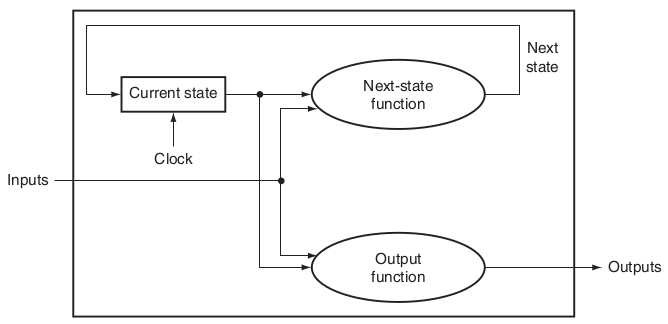
\includegraphics[width=4in]{fsm0.png}
	\caption{A Finite State Machine and its main components.}
	\label{fig:fsm0} 
	\end{center}
\end{figure}

\subsubsection{Example: Traffic Lite}
Let us design a simple traffic light system. The following tables and figures 
contain the specification. 

\begin{table}[h!]
  \begin{center}
    \caption{Outputs.}
    \label{tab:Outputs}
    \begin{tabular}{l|p{4in}} 
      \textbf{Signal} & \textbf{Description}\\
      \hline
      NSLite & When this signal is asserted, the light on the north-south 
      road is green; when this signal is deasserted, the light on the 
      north-south road is red \\ \hline
      EWLite & When this signal is asserted, the light on the east-west road is 
      green when this signal is deasserted, the light on the east-west 
      road is 
      red \\ \hline
    \end{tabular}
  \end{center}
\end{table}

\begin{table}[h!]
  \begin{center}
    \caption{Inputs.}
    \label{tab:inputs}
    \begin{tabular}{l|p{4in}} 
      \textbf{Signal} & \textbf{Description}\\
      \hline
      NScar & Indicates that a car is over the detector placed in the roadbed 
      in front of the light on the north-south road (going north or south) \\ 
      \hline
      EWcar & Indicates that a car is over the detector placed in the roadbed 
      in front of the light on the east-west road (going east or west) red \\
      \hline
    \end{tabular}
  \end{center}
\end{table}

\begin{table}[h!]
  \begin{center}
    \caption{States.}
    \label{tab:states}
    \begin{tabular}{l|p{4in}} 
      \textbf{Signal} & \textbf{Description}\\
      \hline
      NSgreen & The traffic light is green in the north-south direction \\ 
      \hline
      EWgreen & The traffic light is green in the east-west direction. \\
      \hline
    \end{tabular}
  \end{center}
\end{table}


\begin{figure}[H]
	\begin{center}
	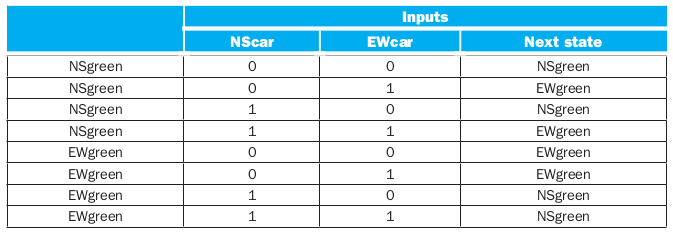
\includegraphics[width=4.5in]{fsm1.png}
	\caption{Next-state function.}
	\label{fig:fsm1} 
	\end{center}
\end{figure}

\begin{figure}[H]
	\begin{center}
	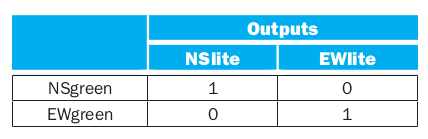
\includegraphics[width=3in]{fsm2.png}
	\caption{Output function.}
	\label{fig:fsm2} 
	\end{center}
\end{figure}

Finite State Machines can be visually represented as State Transition Diagrams 
(STDs). Nodes represent the states. The active outputs for the state are placed
inside the nodes. Directed arcs are used to show the next-state function, with 
labels on the arcs specifying the input conditions as logic functions.

\begin{figure}[H]
	\begin{center}
	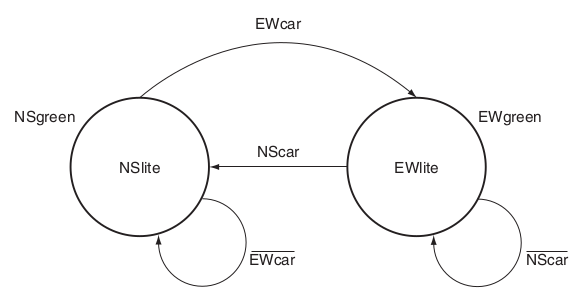
\includegraphics[width=4in]{fsm3.png}
	\caption{State Transition Diagram for Traffic Lite.}
	\label{fig:mux} 
	\end{center}
\end{figure}

The final VHDL Code for the traffic lite is given below.

\begin{minted}[frame=single,framesep=10pt]{vhdl}
LIBRARY ieee;
USE ieee.std_logic_1164.all;
---------------------------------
ENTITY trafficlite IS
   PORT (EWCar, NSCar, clk: IN STD_LOGIC;
      EWLite, NSLite: OUT STD_LOGIC
   );
END trafficlite;
--------------------------------
ARCHITECTURE pure_logic OF trafficlite IS
   SIGNAL state : STD_LOGIC := '0'; 
BEGIN
   PROCESS(clk)
   BEGIN
      NSLite <= NOT state; EWLite <= state;
      IF (RISING_EDGE(clk)) THEN
         CASE state IS
            WHEN '0' =>
               state <= EWCar;
            WHEN '1' =>
               state <= NSCar;
            WHEN others => 
               state <= '0';
         END CASE;
      END IF; 
   END PROCESS;
END pure_logic;
\end{minted}


\section{Summary}
In this lab, you learned some of the sequential elements that are useful in the 
design of a processor as well as the importance of clocks. We also showed the
design and implementation of a simple traffic light system using finite state 
machines since a simple truth table is not enough to characterize a sequential 
system. 

You should now be able to tell whether a functional component of a datapath and 
control is composed of a combinational or sequential element.

\section{Learning Activities}
Download the source codes for this lab then try experimenting by adding more 
test cases in the testbenches. Submit a PDF document that shows screenshots of 
your modifications and runs. 

\section{Self-Assessment Questions}
\begin{enumerate}
\item What is the main purpose of clocks in sequential circuits?
\item What is the difference between a clocked latch and a flip-flop?
\item Why can't a multiplexer be used in RAM?
\item Why is SRAM more expensive than DRAM?
\item If my CPU is clocked at 800 MHz, what is the period?
\end{enumerate}


\section{Deliverable}
Your final deliverable for this lab is implement the RAM in Figure 
 \ref{fig:sram3}. Submit the VHDL code including a testbench as well as images 
of the waveforms. NOTE: Enable lines should be connected to the output of the 
decoder and the rightmost Din in the figure should be Din[0].

\section{Further Reading}
\begin{itemize}
\item 
\href{https://www.doulos.com/knowhow/vhdl/simple-ram-model/}
{https://www.doulos.com/knowhow/vhdl/simple-ram-model/}
\end{itemize}


%\begin{thebibliography}{9}
%\end{thebibliography}

\bibliographystyle{unsrt}
\bibliography{seque}
\nocite{*}

\end{document}